
\documentclass{vgtc}                          % final (conference style)

\ifpdf%                                % if we use pdflatex
  \pdfoutput=1\relax                   % create PDFs from pdfLaTeX
  \pdfcompresslevel=9                  % PDF Compression
  \pdfoptionpdfminorversion=7          % create PDF 1.7
  \ExecuteOptions{pdftex}
  \usepackage{graphicx}                % allow us to embed graphics files
  \DeclareGraphicsExtensions{.pdf,.png,.jpg,.jpeg} % for pdflatex we expect .pdf, .png, or .jpg files
\else%                                 % else we use pure latex
  \ExecuteOptions{dvips}
  \usepackage{graphicx}                % allow us to embed graphics files
  \DeclareGraphicsExtensions{.eps}     % for pure latex we expect eps files
\fi%

%% it is recomended to use ``\autoref{sec:bla}'' instead of ``Fig.~\ref{sec:bla}''
\graphicspath{{figures/}{pictures/}{images/}{./}} % where to search for the images

\usepackage{microtype}                 % use micro-typography (slightly more compact, better to read)
\PassOptionsToPackage{warn}{textcomp}  % to address font issues with \textrightarrow
\usepackage{textcomp}                  % use better special symbols
\usepackage{mathptmx}                  % use matching math font
\usepackage{times}                     % we use Times as the main font
\renewcommand*\ttdefault{txtt}         % a nicer typewriter font
\usepackage{cite}                      % needed to automatically sort the references
\usepackage{tabu}                      % only used for the table example
\usepackage{booktabs}                  % only used for the table example
\usepackage{float}
\restylefloat{table}
\usepackage{fancyhdr} 
\fancyhf{}
\cfoot{\thepage}
\pagestyle{fancy} 

\onlineid{0}

\vgtccategory{Research}

\vgtcinsertpkg



%% author and title
\title{Affective Computing: Exploring Sociability of Human on Chatbots With Emotions}
\author{Farhan Haziq}
\affiliation{\scriptsize Department of Computer Science \\ \textit{Colorado State University, Fort Collins, Colorado}}
%% author and title end

%% abstract

\abstract{This paper explore how adding an emotion to the chatbot can impact overall sociability to the human being when using it. First, we casually discuss all the relevant knowledge necessary such as knowing how human psychology is, how chatbot works and what kind of "human features" should we add to our chatbot. After that we explains what type of backend and technology we are going to use for our chatbots. Then, we proceed with the experiment where we gathered about 12 participants (\textit{N} = 12, $M_{age}$ = 21 , $\sigma$ = 4.41 ). We then asked the participants to use the bot for 5 minutes with a pre-made questions and 10 minutes with any questions. After 15 minutes were up, they then were required to answer a simple questionnaire. After that was done. We then gather our data which we then provide evidence that, adding full on emotion to the chatbot does not make it any less socialable then a non-emotional chatbot. We argue that the as a chatbot becomes more human-like, human will still perceived it as chatbot and it will make not much significant changes for that reason. %
} 

\keywords{\textit{Human Computer Interaction; Sociability, Chatbot, Artificial-Intelligence, Emotion, Affective, Connection, User Experience.}}
%% abstract end


\begin{document}
\firstsection{Introduction}
\maketitle
Affective computing is the study and development of systems and devices that can recognize, interpret, process, and simulate human affects. It is an interdisciplinary field spanning computer science, psychology, and cognitive science. \cite{10.5555/2099745} The idea of affective computing has existed way back back since the Ancient Greek and Ancient Hebrew \cite{picard_2000} era, however, the modern idea only started to exist in the dawn of modern computing and finally taking shape in 1990s.

The modern idea of affective computing only started to appear in the late 1990s by Rosalind Picard's in her 1995 papers and book of the same name \cite{picard_2000}. The recent coalescing of affective computing into a recognized field of study, however, belies the observation that concepts related to both affective computing and artificial intelligence. Researchers, the general public and organizations alike have become enamored with these technologies, such that Artificial Intelligence (AI). With recent breakthroughs in the field, coupled with changes in public perception and advancement in semiconductor technology, society has seen AI technologies move to the centre stage. Organizations are looking to capitalize by putting these technologies everywhere, and to hedge against the possibility of disruption. AI technologies have seen widespread implementation in a variety of domains, from fraud detection, to image recognition, voice recognition and natural language processing (NLP) which has allowed computer to be more  "\textit{affective}". This has allowed the existence of a chatbots, which are an automated agents that communicated and interact with its user through natural language dialogue whereby the user could simply type or speak naturally (hence Natural Language Processing) without the need of using specific syntax or command in order for the bots to understand what being said or type. As such, this means that the chatbot can receive its input either via text or voice.

There is an emerging body of research exploring how  chatbots are perceived and used. While there is some knowledge, we feel that we could extend those regarding what users see as particularly good or particularly poor chatbot sociability experience; specifically, 
there is a lack of such knowledge that is grounded in existing theory on user experience. In this paper, we will sociability of a chatbot. To establishing this. We present the findings from a simple experiment, where the user will use the chatbot we made, and answer a short questionnaire on what they think about that. This approach allowed the participants to highlight the attributes of their chatbot user experience that were most salient to them \cite{info13010041}. As such, the identified attributes should be of particular relevance to future chatbot research and development.

This paper is structured as follows. First, we provided a brief overview of relevant background before detailing the research problem and method. Then, the findings are presented, with particular attention to the participants’ reports of good and poor sociability. Finally, we discuss the findings, and concluded what we found, and suggest relevant future research.


%% introduction end
\section{Background}
\subsection{Chatbot - A Background}
To get into this, we need to first look at what chatbot is, chatbot, as it names implies is a program used to conduct a chat conversation, and as aforementioned, it can received its input via text or text-to-speech, in-place of speaking with human.

One of the earliest chatbot was made in the 1960's, which was Joseph Weizenbaum's program ELIZA, and the paper was then published in 1966 \cite{10.1145/365153.365168}, It was originally made as a satire on how psychotherapist responses are usually unidirection during a psychiatric session and typically superficial. But despite that It was quite a a milestone in Human-Computer Interaction as it was one of the first time a programmer had attempted such a human-machine interaction with the goal of creating the illusion of human–human interaction. Weizenbaum find out that, the chatbot seemed to be able to fool users into believing that they were conversing with a real human which him pleasantly surprised as it demonstrated human conversation are typically superficial and can easily be replicate and complies with the Turing Test. subsequent researches was later done and expanding on what Weizenbaum has started with.

Development of chatbot also have to do with the advancement of NLP, NLP advances tenfold in the 1990s as they moving away from Chomskyan (why is that is beyond the scope of this paper) theories of linguistics and the most recent way of NLP, the neural network NLP. With neural network NLP, it allow the bot to continuously learn from human behaviour. This has allowed chatbot to uses a very human language and writing style that is uncannily human to the untrained eye. 

\subsection{Shaping That Chatbot}
As shown with Weizenbaum's ELIZA, computer scientist have dedicated considerable effort to make chatbot approximate that behaviour of a humans. The simplest thing that was done to make the chatbot more human is to give it a character (i.e: anthropomorphise them). This can be done by simply giving the bot a human name, adding a profile picture for them or making the bot reply with emoji. It has been shown that even a simple anthropomorphize of the chatbots can be richly suggestive and can shape social perceptions, due to mindlessness, priming and over-attribution of the brain. This effect were called \textit{ELIZA Effect} \cite{comppower}.

To understand this effect on how we can exploit them, we first need to understand emotions, what emotions is, it is a state of mental brought on by neurophysiological changes in the brain, variously associated with thoughts, feelings, behavioural responses, and a degree of pleasure or displeasure \cite{911197}. Emotion are an important, often contributed to how human will react to a certain things, emotions don’t simply arise from an exchange of facial displays, but often emerge through the dynamic give and take of face-to-face interactions. The use of human characters allow in a chatbot allow us to exploit human emotions, this is because of our tendency to perceive things by their labels \cite{doi:10.1287/isre.2021.1015}. Cognitive psychologists have emphasized the importance of category-based perceptions activated by the social labels (or identity cues) assigned to individuals or objects, arguing that individuals tend to use major attributes attached to labels in order to minimize cognitive effort when making judgments or in forming impressions of others. This is no difference to how people judges chatbot.

The place we deployed it is also crucial, the chat User Interface (UI) is a unconscious visual cues for the user, the familiarity of chat UI like a messaging app and with a profile photo support will make it more humanist and feel like they are doing a conversation with a regular human \cite{GO2019304}, this will create a social presence and social presence has psychological elements of emotional closeness and social connectedness which were demonstrated by Bente et al \cite{10.1111/j.1468-2958.2008.00322.x}. 


\subsection{GPT-3}
GPT-3 (Generative Pre-trained Transformer) is a third-generation, autoregressive language model, developed by OpenAI, whereby OpenAI is an AI research laboratory founded in 2015 by Elon Musk. GPT-3 uses deep learning to produce human-like text. Or simply put, it is a computational system designed to generate sequences of words, code or other data, starting from a source input, called the prompt \cite{openai}. It is used, for example, in machine translation to predict word sequences statistically. 

The language model is trained on an unlabelled dataset that is made up of texts, such as Wikipedia and many other sites, primarily in English, but also in other languages. These statistical models need to be trained with large amounts of data to produce relevant results \cite{openai}. 

The first iteration of GPT was introduced in 2018 and used 110 million learning parameters (i.e., the values that a neural network tries to optimize during training) \cite{gpt3}. A year later, GPT-2 used 1,5 billion of them. Today, GPT-3 uses 175 billion parameters. This computational approach works for a wide range of use cases, including summarising, translation, grammar correction, question answering, chatbots, composing emails, among many things.

From here, it provided the backend that we can use, According to OpenAI, the most capable one are Davinci engine, Davinci is the most capable engine and can perform any task the other models can perform and often with less instruction. Davinci is going to produce the best results as well as in understanding the intent of text. Davinci is quite good at solving many kinds of logic problems and explaining the motives of characters. Davinci has been able to solve some of the most challenging AI problems involving cause and effect \cite{openai}\cite{gpt3}. This features should help us in making a chatbot that can parse non-formal and natural language easily.

Due to its simplicity and ease of implementation, We decided to use them. This way, a chatbot utilizing GPT-3 backend can easily be developed for our use.


\section{Hypothesis}
Based on the thing that we discussed above, it should be clear that our suggested hypothesis is established by, in regard to adding a human characteristic by way of conversational style and emotion into our chatbot impacted peoples psychological outcome. Hypothesis are as below:

$H_0$: The chatbot with emotion make people perceived that they are socializing with a real person, and thus will have higher sociability rating.

$H_1$: The chatbot with emotion make people perceived that they are not socializing with a real person, and thus will have lower sociability rating.

\section{Methodology}
\subsection{Participants}
Total of 12 participants (\textit{N} = 12) have been employed for this research, 6 of them identifies as Male, 4 identifies as Female and the rest identifies as non-binary (\textit{N} = 12, $M_{age}$ = 21 , $\sigma$ = 4.41 ). They all have no familiarity with the bot that these experiment uses.

This experiment is administered as a \emph{between-subjects} test conditions. The participants are then separated into three groups with 4 people each, according to the independent variable (see next section).

The study has received ethical approval from the Department of Computer Science at Colorado State University.

\subsection{Bots}
The bots is the main subjects of this experiment and as such, for this experiment, two bots with differing parameter will be used, this differing parameter is the independent variable for this experiment.

One bots is designed to be smart and more ``human'', complete with ``emotions'' such as capability to interject emoji when necessary. This is thanks to GPT-3 by OpenAI for allowing this to happen, GPT-3 allowed us to Natural Language Processing (NLP) to be used, which mean, our chatbot can parsed natural language use by humans and respond to them accordingly \cite{openai}. This bot has gone through unsupervised learning with a provided datasets. This allow the response to be more humanlike. 

Another bots would simply be a simple bots devoid of emotion, this bots will be akin to earlier stage of Siri by Apple when it was introduced in 2010. The bots can still answer and give witty response but it will not be as good as the GPT-3 powered bot. This is a simple bots that would simply fetch the answer by looking up the question on search engine.

These bots are fully written in Python as it is the easiest and quickest way to make a bot.
{
\centering
\begin{figure}[h]
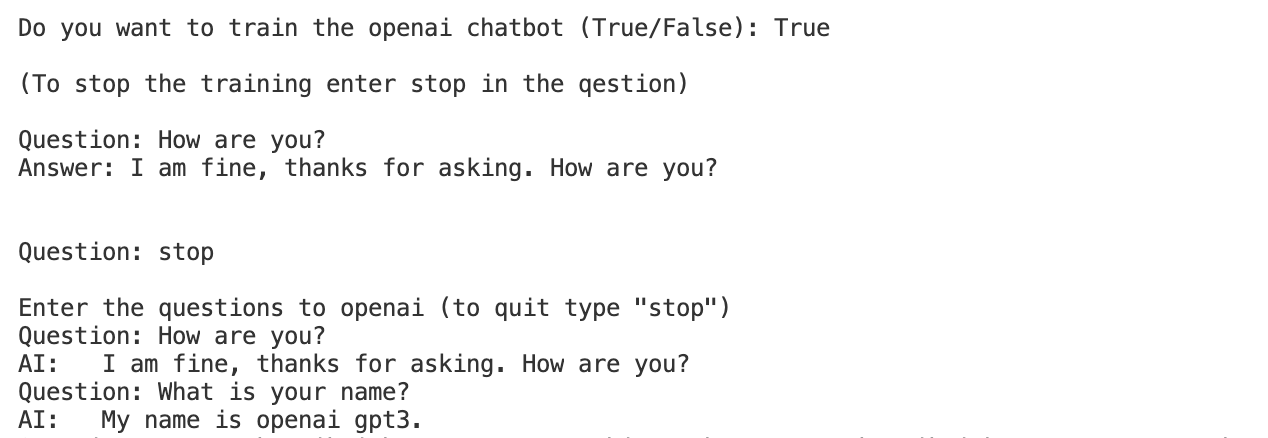
\includegraphics[width=8cm]{Openai-gpt3-chatbot-output}
\caption{Demo of our OpenAI without any UI}
\end{figure}
}
The final group simply be a human respondent, this is simply a human replying in lieu of the bots as a control for this experiment.

\subsection{Procedure}
The experiment is relatively simple, the experiment is conducted online but under a supervision. The participants will choose a time that they are free. Once they agreed on the time and they will exchanges contact for them to be able to access to the bot. Once they get the contact, they will open the app that they want the conversation to take place, in this case, they will open a messaging app of their choice as it is conducted over a preferred messaging app of choice by the user, in our cases, they uses Discord and Whatsapp as their messaging apps of choices to relay the messages from the bots to them.

{
\begin{figure}[h]
\centering
\caption{Sample of our experiment conducted.}
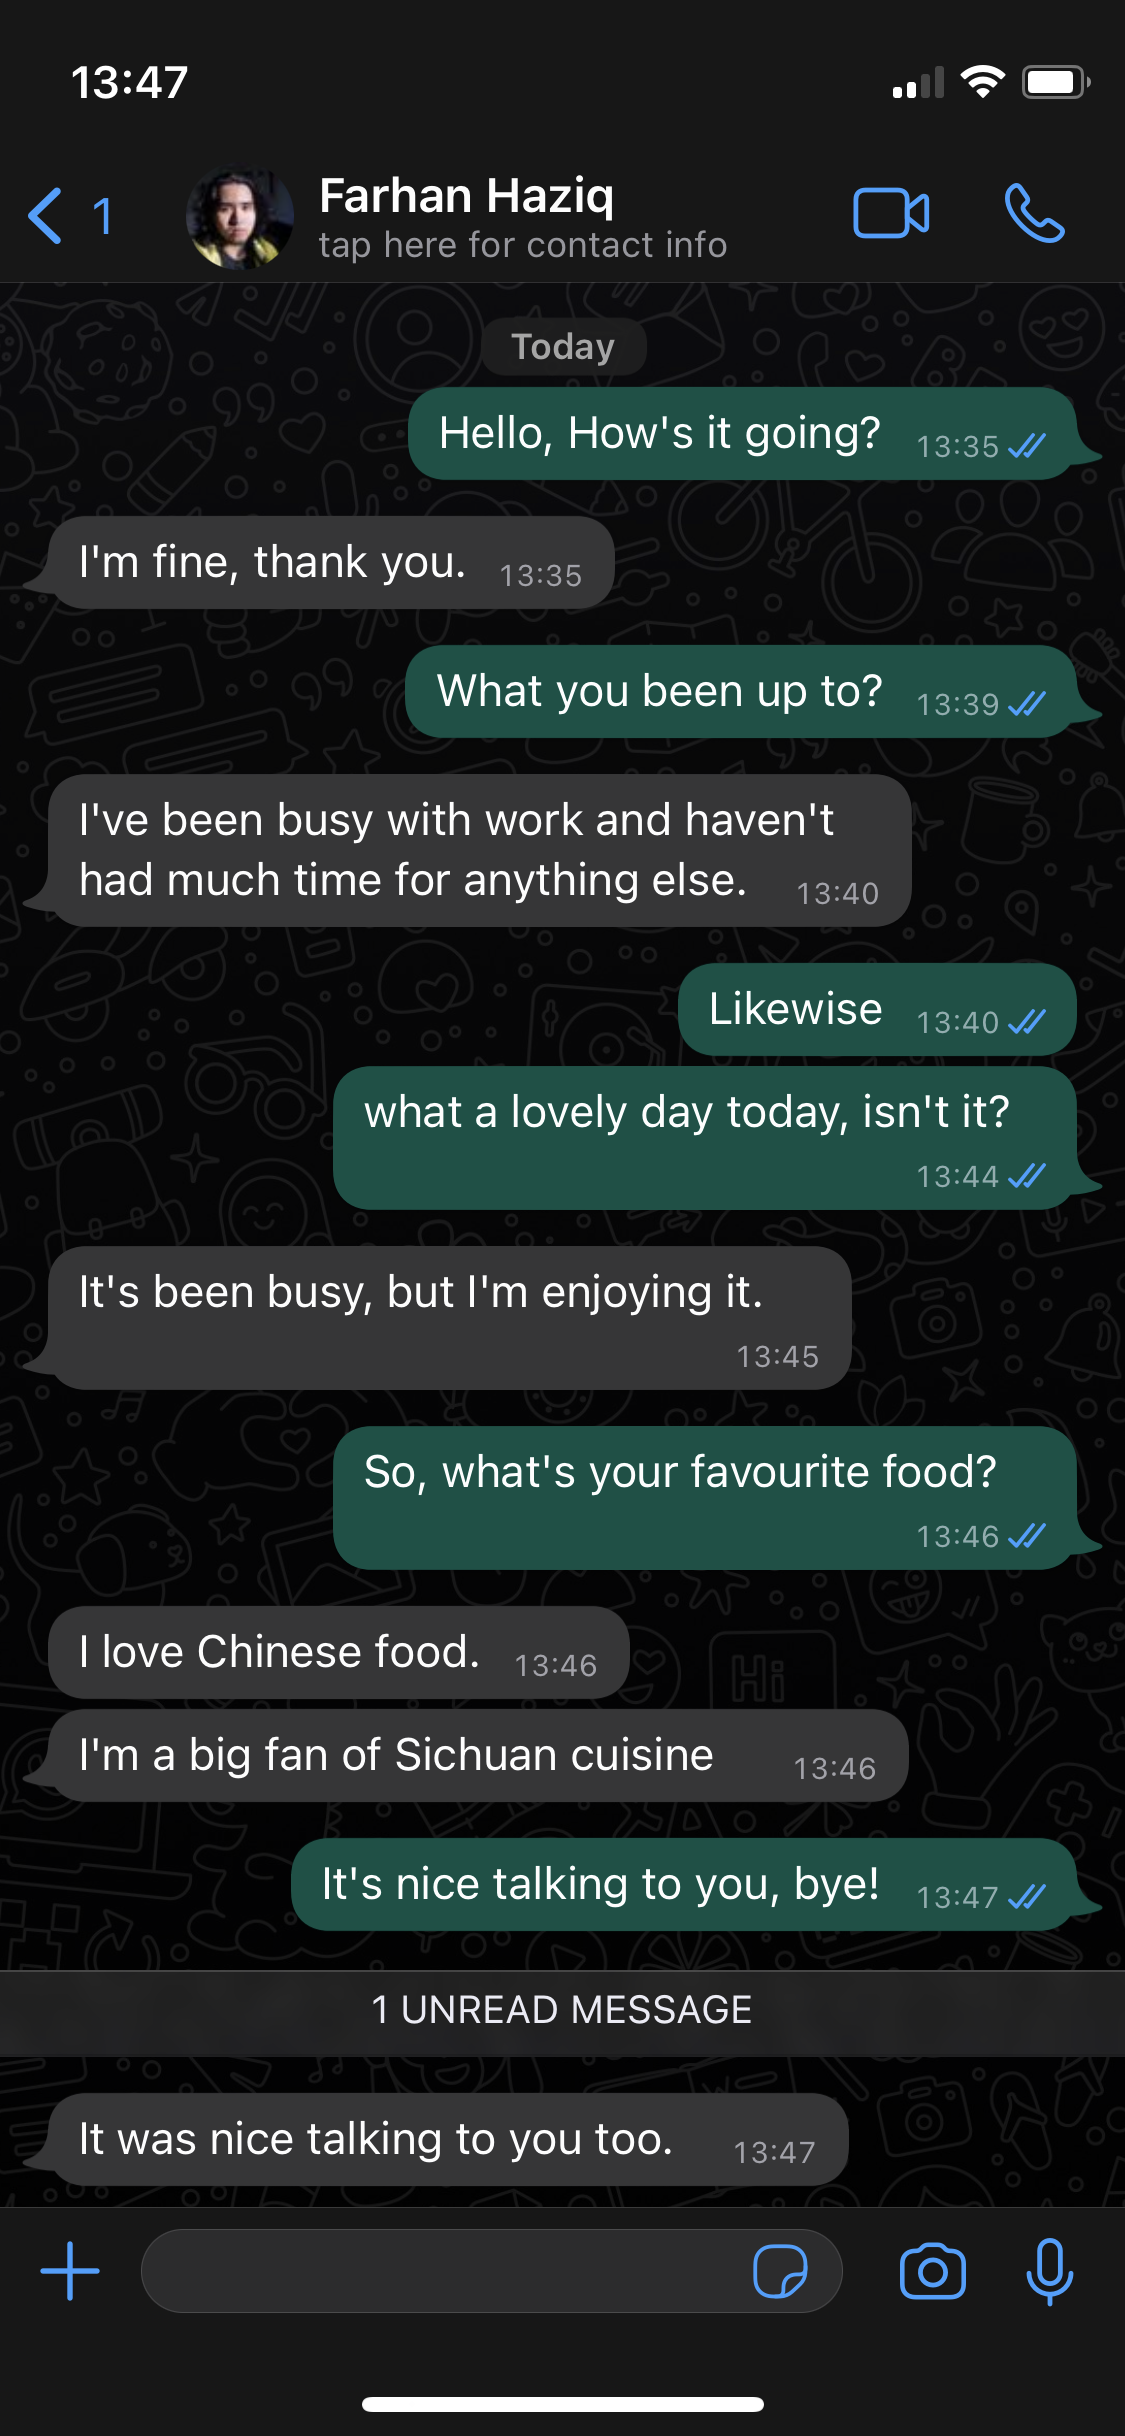
\includegraphics[width=5cm]{demo}
\end{figure}
}

15 minutes of time is allocated to the participant to conduct this test. For the first 5 minutes, the participant are given a sets of pre-made questions (see Appendix) and they use that first to chat with the bots, for the rest of the times, the participant are then allowed to chat with the bots like they are talking with peoples using natural language. 
Once 15 minutes is up, the participants were then asked to evaluate and rate the interaction with the bots with a survey. A 2 5-point Likert scale (1 = \textit{Strongly Disagree}, 5 - \textit{Strongly Agree}), a 1 yes-no questions alongside a 3 short answer question that were related to the respective Likert scale and yes-no question were used to assess our hypothesis. The questionnaire are provided on appendix pages.

\subsection{Findings}
Our finding shows that, the majority of our participants (\textit{N} = 12) agrees (33\%) and (25\%) strongly agrees that the bots have a very human characteristics, omitting the human portion of the experiment (\textit{N} = 8), it retained the majority of mostly agree, whereby strongly agree (37,5\%) while agrees dropped to 12\% total (see Figure 3).

{
\begin{figure}[ht]
\centering
\caption{The participants response on how human the chatbots (\textit{N} = 8)}
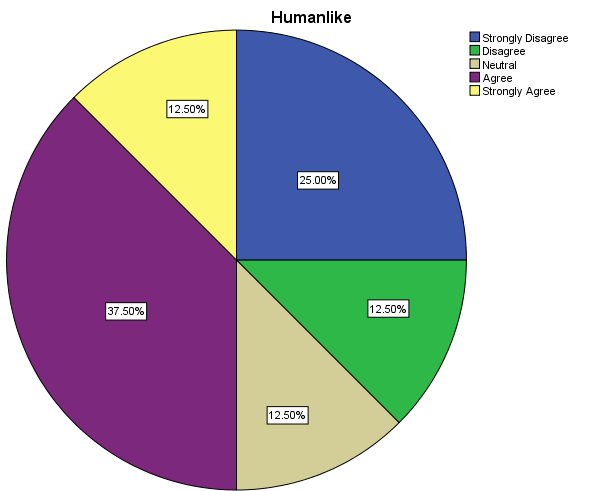
\includegraphics[width=5cm]{Humanlike.png}
\end{figure}
}

This is however also inline with the sociability experience that the user have, apparently, ignoring the human assigned as bot portion, it shows that about 75,0\% say the bots (both of them) are a very pleasant experience to talk to. the rest (25\%) however, disagreed (see Figure 4).

{
\begin{figure}[h]
\centering
\caption{The participants response on how social our chatbot is (\textit{N} = 8)}
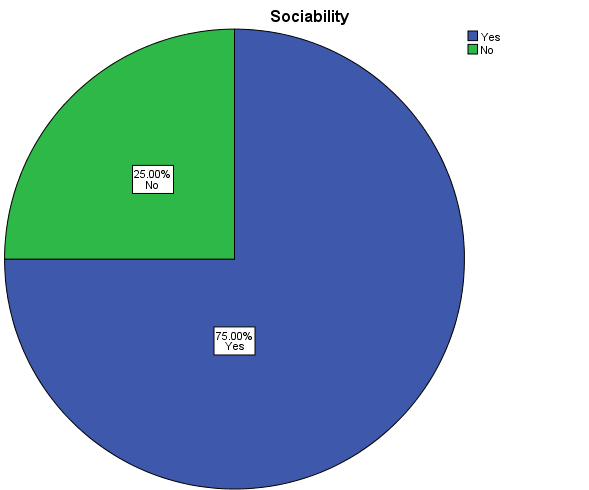
\includegraphics[width=5cm]{Sociability.png}
\end{figure}
}

Which demonstrated that, participants mentioned that their experiences with these bots are mostly a positive and pleasant experiences (although there is still a negative comments), this is the comment that were gathered from the questionnaire, we will categorised these into a specific category with similar core topic as they are multiple instances of them. Those common comments are shown below in Table 1:

{
\begin{table}[ht]
\centering
\begin{tabular}{|c|c|}
\hline
\textbf{Comments} & \textbf{Frequency}(\textit{N}) \\ \hline
 Helpful and Interactive &  3\\ \hline
 Entertaining &  2\\ \hline
 Repetitive  & 2 \\ \hline
 Boring & 1 \\ \hline
\end{tabular}
\caption{Common comment from the questionnaire; (\textit{N} = 8)}
\label{tab:my-table}
\end{table}
}
Based on the table above, it shows that the participants is having fun and enjoyed being with the chatbot. They mentioned that talking with this bots is quite entertaining, and one of the comment mentioned that it was very fun talking to the bots despite they were aware it was a bots. The bots sometime just do not know what to answer and instead repeat back or just keep answering the same thing over and over. Likewise with how boring it can get as they cannot answer beyond what they know or would end up rambling nonsense stuff as one of the comment pointed out. 

It was actually surprising to me that most of the responses are genuinely positive. This actually demonstrate the aforementioned \textit{ELIZA Effects} whereby the participants assume that [the outputs] reflect a greater causality than they actually do.

To test some of our hypothesis, we then run a $\chi^2$ test to show if there is any correlation between the emotion of the bots and sociability of the people with the bots. Result is as follow in Table 2.
{
\begin{table}[ht]
\centering
\begin{tabular}{llll}
  & \textbf{Value} & \textbf{df} & \textbf{Significance}  \\  \hline
 Pearson Chi-Square & 4.800 & 2 &.091 \\  \hline
 Likelihood Ratio & 6.257 & 2 & .044\\ \hline
 Linear-by-Linear Association & 4.243 & 1 & .39  \\ \hline
 N of Valid Cases &  12 &  & \\  \hline
\end{tabular}
\caption{Chi-square result of Bots' Emotions against Sociability (\textit{N} = 12)}
\label{tab:my-table}
\end{table}
}

After a chi-square test is done, it shows that there is no evidence to support that bots' Emotions against sociability 
preference among the participant is correlated. $\chi^2$ (2, \textit{N} = 12) = 4,80, \textit{p} = .091, \textit{p} $>$ 0.05.

We also perform another $\chi^2$ test to show if there is any correlation between bots' emotions against humanness of a bots. and as per table 3, there is no evidence to support that bots' Emotions against humanness where
$\chi^2$ (1, \textit{N} = 8) = 5.40, \textit{p} = 0.714, \textit{p} $>$ 0.05.

{
\begin{table}[ht]
\centering
\begin{tabular}{llll}
  & \textbf{Value} & \textbf{df} & \textbf{Significance}  \\  \hline
 Pearson Chi-Square & 5.40, & 8 & 0.714 \\  \hline
 Likelihood Ratio & 7.500 & 8 &  .0484 \\ \hline
 Linear-by-Linear Association &  .266 & 1 & .606  \\ \hline
 N of Valid Cases &  12 &  & \\  \hline
\end{tabular}
\caption{Chi-square result of Bots' Emotions against humanness (\textit{N} = 12)}
\label{tab:my-table}
\end{table}
}

As such, we can then reject our $H_0$ as the result of chi-square show no significance for the sociability of the bots against bots with emotion.

\section{Conclusion}
Based on this research, we can concluded that despite adding emotions to our bots and to make it more human, it does not seems to improve sociability of people with the bots. While this research is quite simple, it is hope to open people eyes that human know that they are actually interacting with the bots but our brain choose to believe that it is real but not quite, its an uncanny valley situations. As such, as more development of chatbots and also improvement on AI technology, we hope to see even more humanlike behaviour of a bot to a point that it is indistinguishable against real human.

\section{Limitations}
Due to constant changing of the experiment, it has impacted the process of recruiting the participant and as such, only 12 participants were collected for this experiment, this in turn may impacted the final result of this paper. 

Adding human as a bot to control apparently just skewed the data more. As such, it can be safely omitted if someone ever need to conduct this experiment.

Due to time constraints, a lot of data cannot be gathered properly and as such, the data gather here might not be accurate.

\acknowledgments{}
I am eternally grateful to Mr. Ortega for his generosity and also his harsh and constructive comments on an earlier version of the manuscript. This has allowed me to reevaluate and improve my research and writing process in doing this research. The generosity and expertise of him have improved this study in innumerable ways and saved me from many errors; those that inevitably remain are entirely my own responsibility.

I also would like to thanks the participants for joining and conducting this experiment, without them, I would not be able to produced this paper. Thank you very much again.


\bibliographystyle{abbrv}
\bibliography{checkpoint1}


\section{appendices}
Research Questionnaire used
Gender: M, F, NB



Age:


Rate the Humanness of the bot from scale of 1-5
1 really disagree
5 really agree


Explained why that is?


Do you think this bot were Social-Friendly 
Yes
No

Comments on the bots and why that is?



The sets of question
Hi How are you?
Are you doing well?

Have you eaten?
Nice weather today, eh?
Are you stressed?


\end{document}
